%%%%------------------------------
%This document is prepared by 
%--------- Dr. Rudra Pratap Deb Nath -------------------
%--------- Associate Professor---------------------------------------
%----------Department of Computer Science and Engineering----------
%---------- University of Chittagong------------------------
\documentclass[12pt, a4paper]{article}
\usepackage[utf8]{inputenc} %codification of the document

\usepackage{authblk} % This one is for adding affiliation of an author \affil command


%--------------------------
%Package for comment
\usepackage{comment}
%-------------------------------
%Package for coloring text
\usepackage{xcolor}

%---------------------------------

% Package for math

\usepackage{amsmath}
%------------------------------------------

% Package for images

\usepackage{graphicx}


%------------------------------------------

% Package for coding

\usepackage{listings}


%------------------------------------------
% Package for algorithms

\usepackage[ruled,vlined]{algorithm2e}


%------------------------------------------

%%For coloring and linking the reference and url. 
\usepackage{hyperref}
\hypersetup{
    colorlinks=true,
    linkcolor=blue,
    filecolor=magenta,      
    urlcolor=blue,
    pdftitle={Sharelatex Example},
    bookmarks=true,
    pdfpagemode=FullScreen,
}
%%---------------------------------
%% A macro is a shorthand for a more complicated sequence of commands. Later in the text, the macro can be used instead of those sequence of commands. 

\newcommand {\pr}{\textit{Projection,}$\pi$}
\newcommand {\se}{\textit{Selection,} $\sigma$}
\newcommand {\cp}{\textit{Cartesian product,}$\times$}
\newcommand {\un} {\textit{Union,}$\cup$}
\newcommand {\di}{\textit{Set difference,}$-$}
\newcommand {\re}{\textit{Rename,}$\rho$}

%----------------------------

%\begin{center}
%A thesis submitted to the Technical Faculty of IT and Design at Aalborg University (AAU) and the Department of Service and Information System Engineering at Universitat Politècnica de Catalunya (UPC), in partial fulfillment of the requirements within the scope of the IT4BI-DC programme for the joint Ph.D. degree in Computer Science. The thesis is not submitted to any other organization at the same time.
%\end{center}


%-------------------------


%-------------------------------
\begin{document}

\begin{titlepage}

\begin{figure}
	\centering
	\begin{minipage}[b]{0.15\textwidth}
		
\includegraphics[width=1\textwidth]{images/cu}
		%\caption{Black Image}
	\end{minipage} \hfill
	\end{figure}
	
\noindent%
  \begin{tabular}{@{}p{\textwidth}@{}}
    \hline
    \hline
    \vspace{0.2cm}
    \begin{center}
    \Huge{\textbf{
      FLAT MANAGEMENT SYSTEM % insert your title here
    }}
    \end{center}
    \vspace{0.2cm}\\
    \hline
    \hline
  \end{tabular}
  \vspace{4 cm}

\begin{center}
    {\large
      Database Project Report %Insert document type (e.g., Project Report)
    }\\
    \vspace{0.2cm}
    {\Large
      Group-11 % Insert group number
      
    }
  \end{center}
  \vfill
  
  \begin{center}
  Report submitted April 03, 2022
  \end{center}
	\vfill
A project submitted to Dr. Rudra Pratap Deb Nath, Associate Professor, Department of Computer Science and Engineering, Chittagong University (CU) in partial fulfillment of the requirements for the Database Systems Lab course. The project is not submitted to any other organization at the same time. 

\end{titlepage}
\clearpage
%%%% Details of student
%-------------------------
%Fill up the table with your group information
%----------------------------

\begin{table}[t]
\caption{Details of Group-11}% insert your group number 
\resizebox{\textwidth}{!}{%
\begin{tabular}{|l|l|l|l|l|}
\hline
Roll Id & Name & Sigature & Date & Supervisor Approval \\ \hline
      &      &          &      & keep it blank                   \\ \hline
19701075 & Talhabin Siam & Md Siam & 03-04-2022&
                \\ \hline
      19701044  &Jahangir Alam Jehad      &  Jehad        &03-04-2022      &                     \\ \hline
     19701074   & Abu Noman Shawn Sikder    & Shawn         & 03-04-2022     &                     \\ \hline
     19701071   & Rabbi Hasan     &  Rabbi        &  03-04-2022   &                    \\ \hline
      19701059  &  Md Hasan Mia    &  Hasan        & 03-04-2022    &                     \\ \hline
\end{tabular}%
}
\end{table}
\clearpage






%-------------------------

% Showing contents as an Index
\setcounter{secnumdepth}{5}
\setcounter{tocdepth}{5}
\tableofcontents
\listoffigures

\listoftables
\lstlistoflistings
%-----------------------







\begin{abstract}
    



\noindent
%Explain the following points: Why are you doing this database project? What is the problem you choose? Why does it motivate you? What are current problems faced by the stack-holders? What solution will your system provide? What are the process you will use to develop your solution? The significance of your project, limitation and future work in short
We chose the flat management  system. Many of renters are facing problems when  searching  a flat, cottage or mess. Also flat owner can easily handle their flats, cottages. People can easily see the flats and 
find their expected flats. Also mess manager can add room when there is a vacancy in his/her mess.
For solving  this system we chose the flat management system.

\end{enumerate}


\end{abstract}

\clearpage

% Maintain the consistency.
% Maintain a good writing flow. 

\section{Introduction}\label{sec:introduction}
We are exercising this project for learning easy management of flat. The objective of this course is to develop a database application system by applying the theories, methodologies, tools, and technologies we are learned in Database System[CSE-413].

\subsection{Background and Motivation}\label{subsec:bm}
This project is highly important for us to overcome the limitations of the manual data
management system. On account of this problem many companies & organizations lose  their precious time and money. Currently it is really difficult to manage a large amount
of data and search a particular data. Our project can solve the limitations
easily. Because of this process time will be saved and so money will be saved.

\subsection{Problem Statement}\label{subsec:ps}
The Flat Management system is developed for making it easy to find the cottage/mess/flat. This system will contain all information about cottages/messes/flats from where customers can find out their preferable cottages/messes/flats according to their budgets/ choices. Users can perform different kinds
of queries based on their location preferences, budget etc.
\subsection{System Definition}\label{subsec:sd} 
Flat Management system  is used for managing the cottage/mess/flat virtually which can store information about cottages/messes/flats in where customers can easily find out their expected cottages/messes/flats.

A system definition example of a Conference planning system

\textit{``A computerized system used to control the ICCIT conference by registering participants and their payments to organizers using invoicing and other reporting methods. Controlling should be easy to learn, as ICCIT conferences use unpaid and untrained labor."}
\newpage
\noindent
\subsection{System Development Process}\label{subsec:sdp}
We  are following several steps. At first, we collect requirements. Then we
analyze requirements and find some entity types and attributes. With those
entity types and attributes we form an Entity Relationship(ER) diagram. After that we map it onto a relational schema. Then we normalize our database. For developing this system we use PHP as backend language and javascript, HTML, CSS, Jquery for designing frontend.
\begin{comment}


To design a database, one should follow the following steps:
\begin{enumerate}
\item Requirement analysis
	\begin{itemize}
		\item[-] interviewing, documentation, etc .
	\end{itemize}

\item Mapping onto a conceptual model (conceptual design)
     \begin{itemize}
     	\item[-] Entity Relationship(ER) model
     \end{itemize}
\item Mapping onto a data model (logical design)
	\begin{itemize}
     	\item[-] Relational model, object model etc. 
     \end{itemize}
\item Normalization
\item System Architecture
\item Realization and Implementation (physical design)    
    
\end{enumerate}
\end{comment}


\subsection{Organization}  Section~\ref{sec:introduction} gives the overview of the project, Section~\ref{sec:projectmanagement} describes how the project and the resources are managed.
Section~\ref{sec:rga} describes how requirements are gathered and analysed.
Section~\ref{sec:cm} describes how we model our database using Entity Relationship(ER) model, Section~\ref{sec:lm} describes how we convert
our Entity Relationship(ER) model into Relational model, Section~\ref{sec:norm} describes functional dependencies of each relation schema from previous, Section~\ref{sec:lm} and shows that
they are normalized up to 3NF or BCNF, Section~\ref{sec:ncp} describes the overall
architecture of our database system, Section~\ref{sec:sa} describes the whole process of front end and back end of our database system, Section~\ref{sec:imp} describes the success of our product and manual of the system for users, Section~\ref{sec:val} describes the formal proof and disclosure of Flat  Management System, Section~\ref{sec:sd} describes how to install and configure our system so that a non-technical user can use
our system, Finally, the conclusion and the pointers to future work is outlined in section~\ref{sec:cfw}.

\clearpage
\section{Project Management}\label{sec:projectmanagement}
Our team consists of 5 members. On completion of different virtual meeting we selected Flat Management System as our database  management system project.\\
\textbf{Project Leader : Md Siam}\\
\textbf{Requirement Analysis :}
\begin{enumerate}
    \item Md Siam
    \item Rabbi Hasan
    \item Abu Noman Shawn Sikdar
    \item Jahangir Alam Jehad
    \item Hasan Mia
\end{enumerate}
\textbf{ER Diagram}
\begin{enumerate}
    \item Md Siam
    \item Rabbi Hasan
    \item Abu Noman Shawn Sikdar
\end{enumerate}
\textbf{Logical Modeling}
\begin{enumerate}
    \item Md Siam
    \item Rabbi Hasan
    \item Md Hasan Mia
    
\end{enumerate}
\textbf{Normalization}
\begin{enumerate}
    \item Rabbi Hasan
    \item Md Siam
    \item Jahangir Alam Jehad
    \item Md Hasan Mia
    \item Abu Noman Shawn Sikdar
\end{enumerate}
\newpage
\noindent
\textbf{System deployment : Database setup in pc}
\begin{enumerate}
    \item Md Siam
    \item Jahangir Alam Jehad
\end{enumerate}
\textbf{Backend:}
\begin{enumerate}
    \item Md Siam
    \item Md Hasan
\end{enumerate}
\textbf{Database:}
\begin{enumerate}
    \item Md Siam
    \item Rabbi Hasan
    \item Abu Noman Shawn Sikdar
    \item Jahangir Alam Jehad
    \item Hasan Mia
\end{enumerate}
\textbf{Front-end :}
\begin{enumerate}
    \item Jahangir Alam Jehad
    \item Abu Noman Shawn Sikdar
    \item Md Hasan Mia
    \item Md Siam
    \item Rabbi Hasan\\
\end{enumerate}
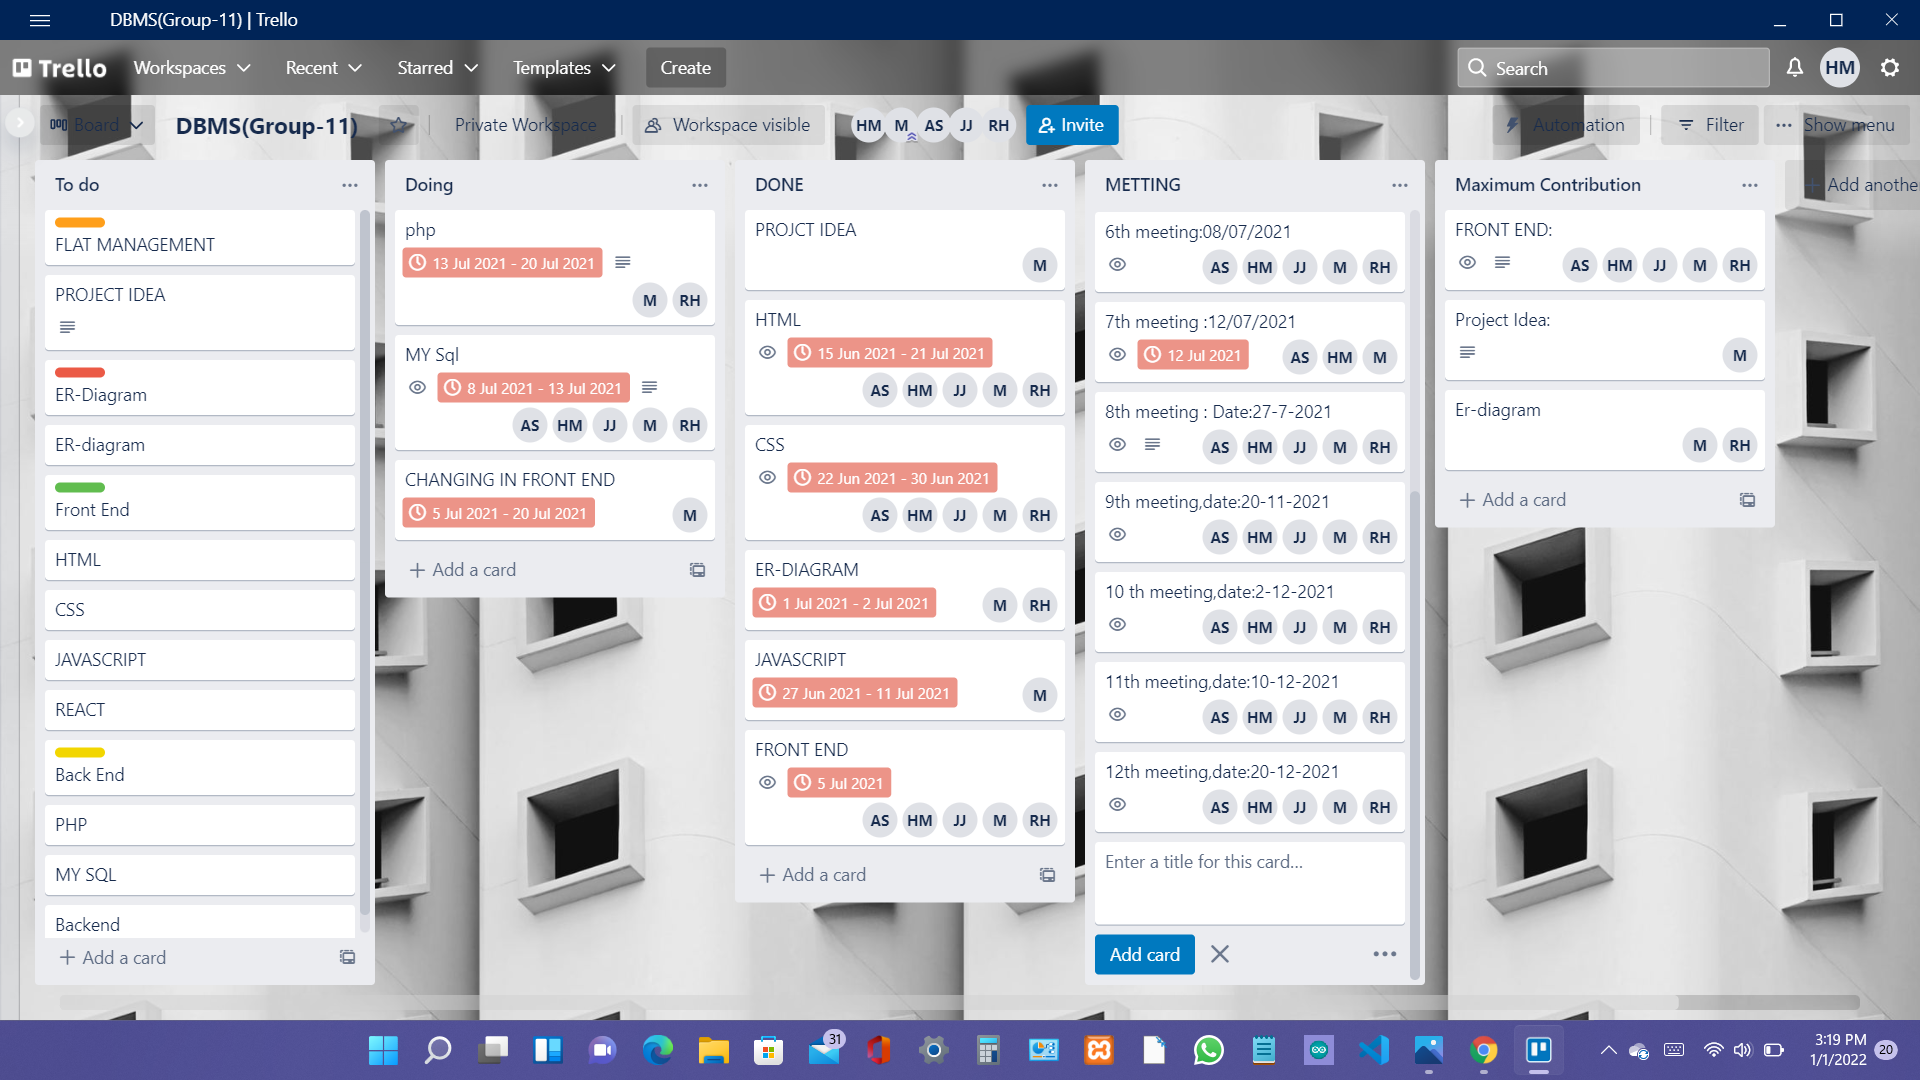
\includegraphics[width=1\textwidth, inner]{trello1.png}
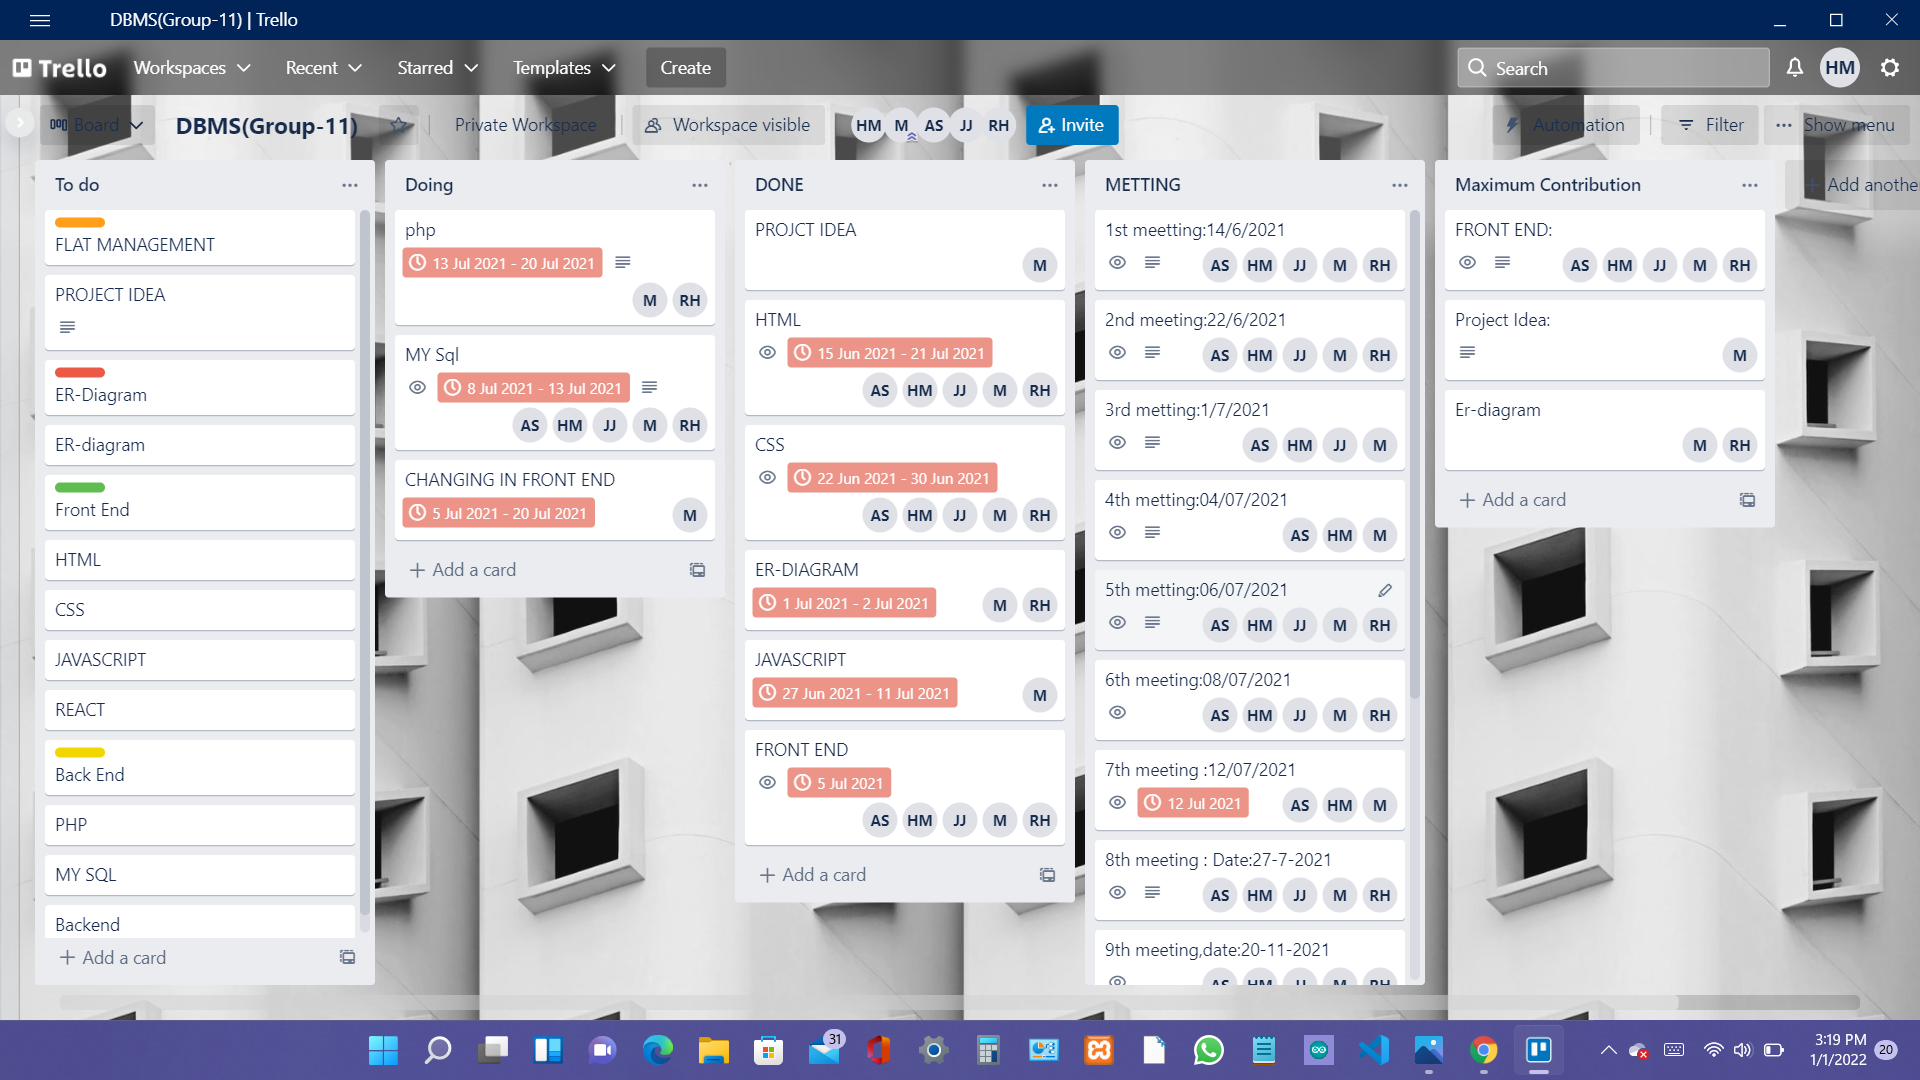
\includegraphics[width=1\textwidth, inner]{trello2.png}
\begin{center}
    Figure: Group meeting and schedule using "Trello" software.
\end{center}

\clejearpage
\section{Requirement Gathering and analysis}\label{sec:rga}
 University Students  are our stackholders who are sharing their problems when they are searching the flat, cottage or mess for renting.
Our team members are talking face to face with different university students 
 to gather information for our project requirement.\\
\textbf{Requirement : }
\begin{enumerate}
     

\item Flat owner section
\item Renter/general user section
\item Admin section
\item Renter can search flats with a filter.
\item Renter can request for booking flats.
\item Admin can add, remove and update user.
\item Admin can see all users and  flats.
\item Flat owners can add ,remove and update flats.
\item Flat owners can see all requests for a flat.
\item Flat owners can see  the booked and unbooked users.
\end{enumerate}
\textbf{System Requirement : }
\begin{enumerate}
    

\item HTML
\item CSS
\item BOOTSTRAPhttps 
\item JAVASCRIPT
\item JQUERY
\item Mysql
\item XAMPP(Apache) 
\end{enumerate}
\clearpage 
\section{Conceptual Modelling}\label{sec:cm}
%Conceptually model your database using an E-R diagram. Use the legends in your diagram. Write how you find the entity types, relationships, and attributes from Section~\ref{sec:rga}
\textbf{ER} Diagram stands for Entity Relationship Diagram, also known as \textbf{ERD} is a diagram that
displays the relationship of entity sets stored in a database. In other words, ER diagrams help to explain the logical structure of databases. ER diagrams are created based on
 three basic concepts: entities, attributes and relationships.
 \begin{enumerate}
    
\item Entity type: A group of definable things, such as User, whereas the entity would be the specific User. 
\item Entity set: Same as an entity type,but defined at a particular point in time, such
as User registration first day of the month.
Relationship: How entities act upon each other or are associated with each other.
\item Attribute: A property or characteristic of an entity. Often shown as an
oval or circle.
\item Cardinality: Defines the numerical attributes of the relationship between
two entities or entity sets . The three main cardinal relationship are (1).one-to-one,(2). 
one-to-many and (3).many-to-many.\\
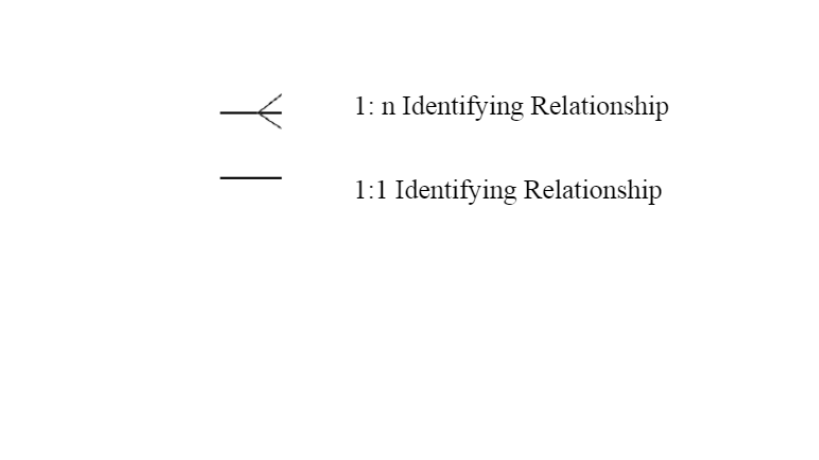
\includegraphics[width=1\textwidth, inner]{relationship.png}\\
According to requirements, we have to store about the admin, flat-owner, flat, facilities and renter. Finally, we find here 5 entity types like General User, Flat Owner, Admin, Flat, Facilities.

    

%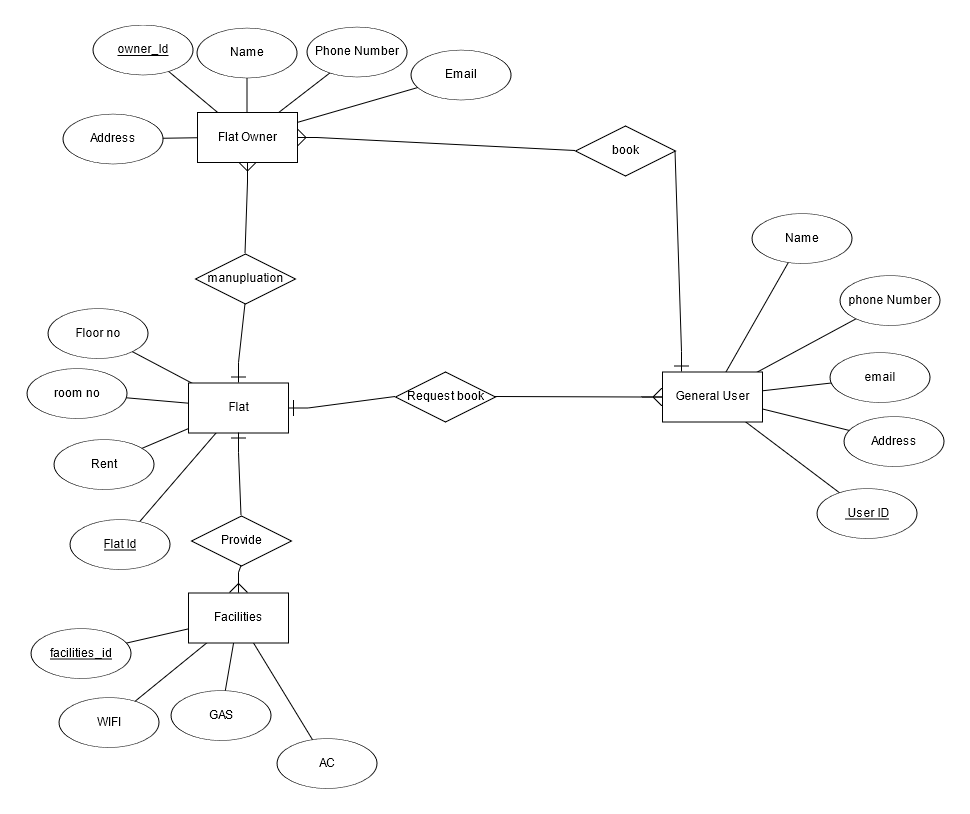
\includegraphics[width=1\textwidth,inner]{images/erdiagram.png}\\
%\begin{center}
   % Fig 1.1:ER Diagram
%\end{center}
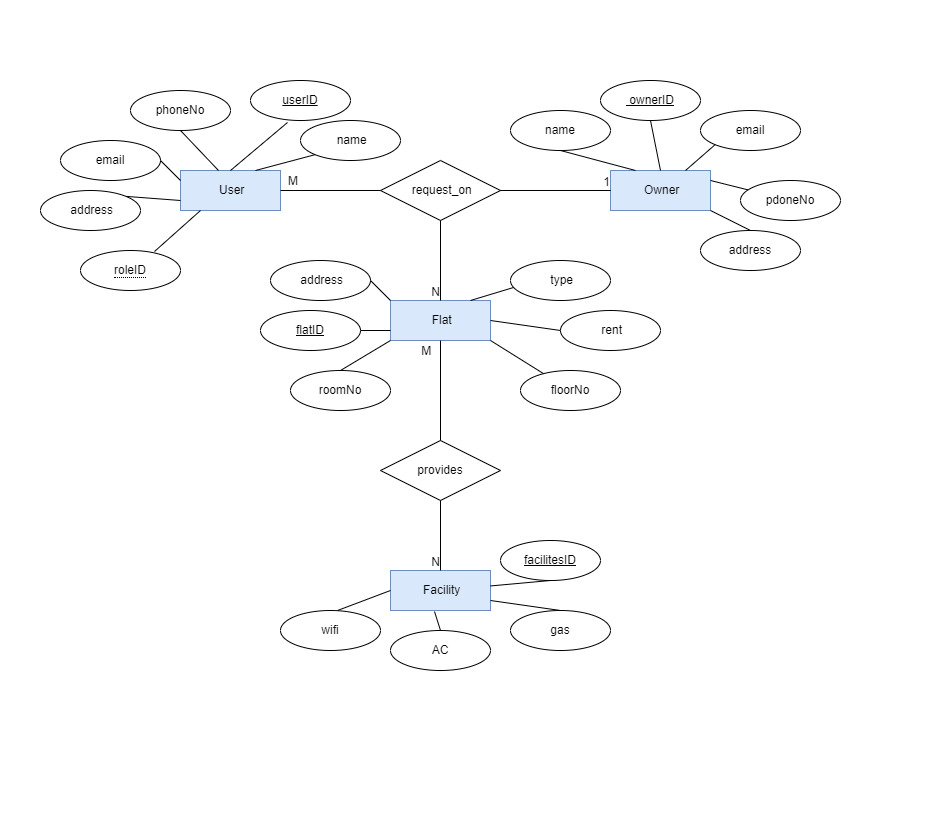
\includegraphics[width=1\textwidth,inner]{images/_erd.drawio.jpg}\\
\begin{center}
    Figure-1: Entity Relationship(ER) Diagram.
\end{center}
 
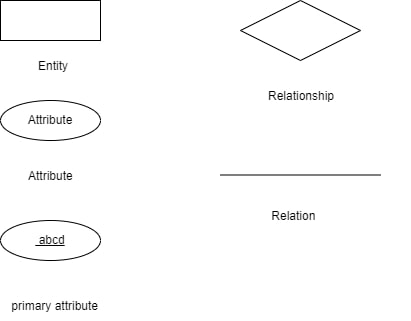
\includegraphics[width=1\textwidth,inner]{images/_ Legends used for ER diagram01.drawio.jpg}\\
 \begin{center}
    Figure-2: Legends used for ER diagram.
\end{center}


 \end{enumerate}    
 \\
 \\
 \newpage
 \noindent
 \textbf{Unary relationship (recursive):}
A unary relationship, also called recursive, is one in which a relationship exists between occurrences of the same entity set. In this relationship, the primary and foreign keys are the same, but they represent two entities with different roles.
 \\
 \\
 \textbf{Binary relationship:}
 When there are exactly two  entity sets participating in a relationship then such type of relationship is called binary relationship.\\
 \\
 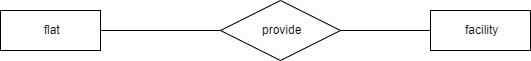
\includegraphics[width=1\textwidth,inner]{images/Binary relationship.drawio.jpg} 
 \begin{center}
    Figure-2.1: Binary Relationship.
 \end{center}
  
 \\
 \\
 \noindent
 \textbf{Ternary relationship:}
A ternary relationship is an association among three entities. This type of relationship is required when binary relationships are not sufficient to accurately describe the semantics of the association. The ternary relationship construction is a single diamond connected to three entities as shown in Figure2.2.\\
 \\
 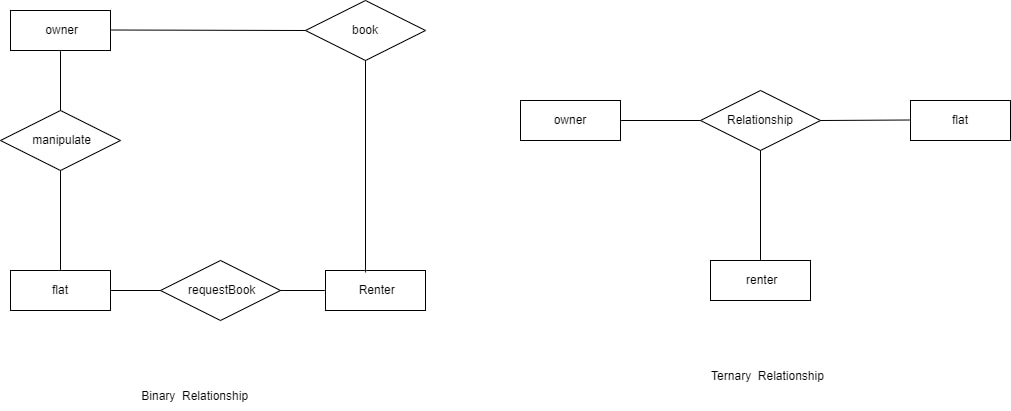
\includegraphics[width=1\textwidth,inner]{images/Untitled Diagram.drawio.jpg}
 \begin{center}
     Figure-2.2: Ternary Relationship 
 \end{center}
 
 
  
\section{Logical Modelling}\label{sec:lm}
A logical data model establishes the structure of data elements and the relationships among them. The relational data model provides a standard way of representing and querying data that can be used by any application. At the beginning, developers can recognize that the main strength of the relational database model is in its use of tables, which is an intuitive, efficient and flexible way to store and access structured information.\\
\noindent
\textbf{This logical model captured from \textit{phpMyadmin} which is formed by
our established database:}\\
\begin{figure}
\centering
 
    
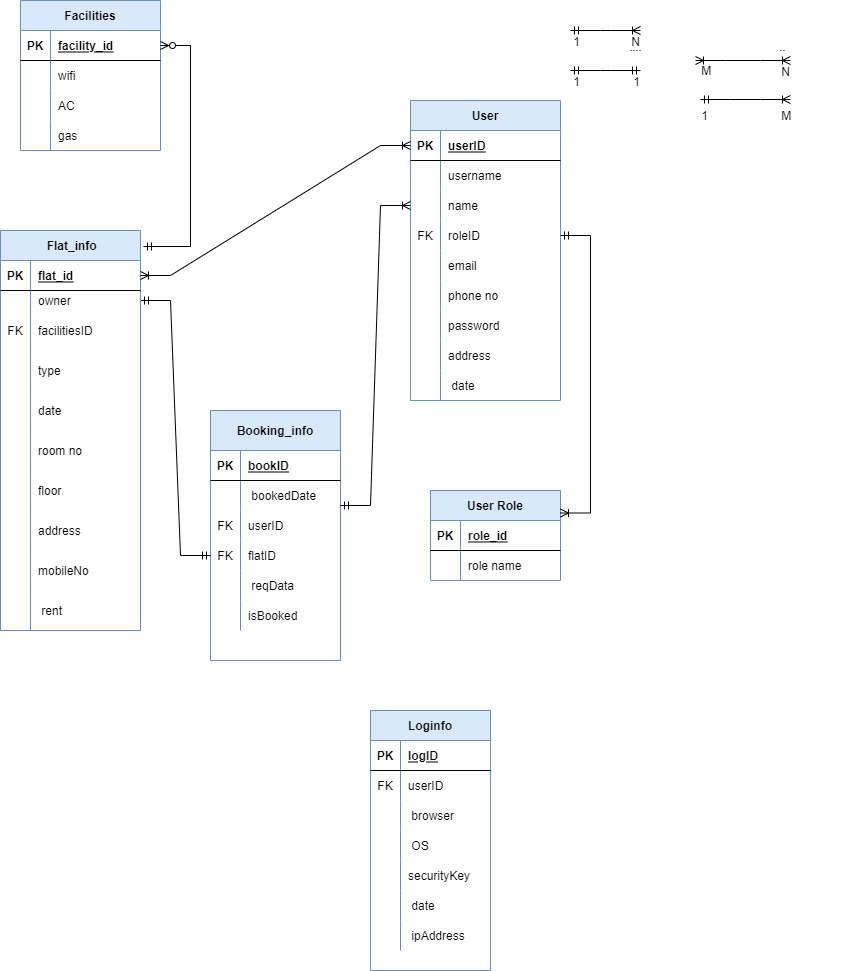
\includegraphics[width=1\textwidth, inner]{images/RM.png}\\
\begin{center}
 Figure-3: Relational modeling
\end{center}
\end{figure}
\clearpage
\section{Normalization}\label{sec:norm}
%From your Relational model, find the functional dependencies of each relation schema and show that they are normalized upto 3NF or BCNF.%
Normalization is a process of avoiding as possible redundancy from a relation or a set of relational table . Redundancy may occur many problems like \begin{enumerate}
\item Insertion anomalies
\item Deletion anomalies and 
\item Updating anomalies.
\end{enumerate}
\\
 
\noindent  
\textbf{Insertion anomalies : }An insertion anomaly is the unability to add data to the database due to the absence of other data . Suppose,a new  Flat-ID is inserted into flat-Info table but won't insert  data under the tuple then the data is made inconsistencies due to omission in database.\\

\noindent
\textbf{Deletion anomalies : }A deletion anomaly occurs when you delete a record that may contain attributes that shouldn’t be deleted. For instance,if we delete an record in an attributes , we will have a chance to loss  other attributes information in  a corresponding table .\\
\noindent
\textbf{Updating anomalies : }An update anomaly is a data inconsistency that results from data redundancy and a partial update .
\\
So,normalization  helps to eliminate this type problem and  makes it easier  to retrieve data.

\subsection{First Normal Form(1NF)}
"A relation does not contain any multi-valued attributes and composite attributes." In first normalization,
\begin{enumerate}
\item There are only Single Valued Attributes.
\item Attribute Domain does not change
\item There is a unique name for every Attribute/Column.
\item The order in which data is stored does not matter.
\end{enumerate}
 
\\
\noindent
 \textbf{Multi-valued attributes} : A multi-valued attribute of an entity is an attribute that can have more than one value associated with the key of the entity. For example , a large company can have many divisions, some of them possibly in different cities.
 \\
\noindent 
\textbf{Composite attributes} : An attribute composed of many other attributes is called as composite attribute.
 \\
 
 \subsection{Second Normal Form(2NF)}
 Second Normal Form (2NF) is based on the concept of full functional dependency . Second Normal Form applies to relations with composite keys , that is, relations with a primary key composed of two or more attributes . A relation with a single-attribute primary key is automatically in at least 2NF .
 In second normal form
 \begin{enumerate}
     \item It must be 1st normal form and
     \item There must be no  partial dependency .
\end{enumerate}
\noindent     
 \textbf{Partial Dependency : }If the proper subset of candidate key determines non-prime attribute, it is called partial dependency\footnote{src-geekforgeek.com/....}.
  
 \subsection{Third Normal Form(3NF)}
 A relation is in third normal form , if there is no transitive dependency for non-prime attributes as well as it is in second normal form .
A relation is in 3NF\footnote{3NF:For each FDs,LHS must be CK/SK OR RHS is a prime attributes }. if at least one of the following A→B:
  \begin{enumerate}
  
 \item It must be 2NF.
 \item There must not be any transitivity and
\item A→B is trivial where $ A \subset R and B \subset R $.
\end{enumerate}
 \\
 \textbf{Transitivity : } If A→B and B→C are two functional dependencies  ,then A→C is called transitive dependency/transitivity . 
 \\
\subsection{Boyce-Codd Normal Form(BCNF) : }
Boyce–Codd Normal Form (BCNF) is based on functional dependencies that take into account all candidate keys in a relation; however, BCNF also has additional constraints compared with the general definition of 3NF.\\
In BCNF:
\begin{enumerate}
\item It must be 3NF .
\item A→B is trivial where$ A \subset R and B \subset R $ . and
\item There must be a super key(SK).
  
\end{enumerate}
\section{Normalization: in the context of project}\label{sec:ncp}
\textbf{KEYS : }
Keys in DBMS is an attribute or set of attributes which helps to identify a row(tuple) in a relation . They allow   to find the relation between two tables . Keys help   uniquely identify a row in a table by a combination of one or more columns in that table . Key is also helpful for finding unique record or row from the table . Database key is also helpful for finding unique record or row from the table.
\begin{enumerate}
 
\item
\textbf{Super Key : }A super key is a group of single or multiple keys which identifies rows in a table.\\
 
\item
\textbf{Primary Key : }A Primary key is a column or group of columns in a table that uniquely identify every row in that table.\\
 
\item
\textbf{Candidate Key : }A Candidate key is a set of attributes that uniquely identify tuples in a table. Candidate Key is a super key with no repeated attributes .\\
\item
\textbf{Alternate Key : } An Alternative key is a column or group of columns in a table that uniquely identify every row in that table.\\
\item
\textbf{Foreign Key : }A Foreign Key is a column that creates a relationship between two tables. The purpose of Foreign keys is to maintain data integrity and allow navigation between two different instances of an entity .\\
\item
\textbf{Compound Key : }A Compound key has two or more attributes that allow you to uniquely recognize a specific record. It is possible that each column may not be unique by itself within the database .\\
\item
\textbf{Prime Attribute : }A prime attribute of the database tables which are candidate keys of the database tables are called prime attributes.\\
\newpage
\item
\textbf{Functional Dependency :}
A functional dependency is a constraint that specifies the relationship between two sets of attributes where one set can accurately determine the value of other sets. It is denoted as X → Y, where X is a set of attributes that is capable of determining the value of Y. The attribute set on the left side of the arrow, X is called Determinant, while on the right side, Y is called the Dependent.

\end{enumerate}
\textbf{Table:User/SignUp}\\
User\{ \underline{userID} , email, username , phoneNo
, name , password , date , roleID , address. \}\\
\newline
Functional Dependency :F\textsuperscript{+} clouser
\begin{enumerate}
\item
\{userID\}→\{username , email , phoneNo , name , date , address.\}\\
\end{enumerate}
Candidate Key : userID..\\
Prime Attribute : userID.\\
Non prime Attribute:email,phoneNO username , name , password , date , roleID , address.\\
Foreign Key : roleID.\\
 
\begin{enumerate}

\item No multi-valued/composite attributes,So it's 1NF.
\item  There is no partial dependency,So it's 2NF.
\item Here,the right side attributes userID is super keys and there is no transitivity/transitive dependency,So it's 3NF.\\
\end{enumerate}\\

\newpage
\noindent
\textbf{Table : FlatInfo}\\
FlatInfo\{\underline{flatID} , owner , type , floor , room , facilitiesID ,address\}\\
\newline
Functional Dependency :F\textsuperscript{+} clouser
\begin{enumerate}
\item 
 
\{flatID\}→\{owner , type , floor , room , facilitiesID , address\}\\
\end{enumerate}
Candidate Key : flatID\\
Prime Attribute : flatID\\
Non prime Attribute : owner , type , floor , room , facilitiesID , address\\
Foreign Key : facilitiesID\\
\begin{enumerate}
\item No multi-valued/composite attributes,So it's 1NF.
\item Single Primary Key and no partial dependency,So it's 2NF.
\item There is no transitivity,So it's 3NF.\\
\end{enumerate}
 
\noindent 
\textbf{Table:LogInfo}\\
LogIn\{\underline{logID} , userID ,ipAddress , browser , OS , password , data\}\\
\newline
Functional Dependency : F\textsuperscript{+} clouser
\begin{enumerate}
\item 
 
\{logID\}→\{userID , ipAddress , browser , OS , password , data\}
\end{enumerate}
Candidate Key: logID\\
Prime Attribute : logID\\
Non Prime Attribute : userID , ipAddress , browser , OS , password , data\\
Foreign Key:userID\\
 
\begin{enumerate}
\item No multivalued/composite attributes,So it's 1NF.
\item Single Primary Key and no partial dependency,So it's 2NF.
\item There is no transitive dependency,So it's 3NF.\\
\end{enumerate}

\newpage
\noindent
\textbf{Table:UserRole}\\
UserRole(\underline{roleID},role\textunderscore{name})\\
\newline
Functional Dependency : F\textsuperscript{+} clouser 
\begin{enumerate}
\item 
\{roleID\}→\{role\textunderscore{name}\}
\end{enumerate}
Primary Key : roleID\\
Prime Attribute : roleID\\
Non Prime Attribute : role\textunderscore{name}\\
\begin{enumerate}
\item No multivalued/composite attributes,So it's 1NF.
\item Single Primary Key and no partial dependency,So it's 2NF.
\item There is no transitive dependency,So it's 3NF.\\
\end{enumerate}

\noindent
\textbf{Table:Facility }\\
Facility\{\underline{facilitiesID},wifi,AC,gas\}\\
\newline
Functional Dependency : F\textsuperscript{+} clouser
\begin{enumerate}

\item 
\{facilitiesID\}→\{wifi , AC , gas\}
\end{enumerate}
Candidate Key/Primary Key : facilitiesID\\
Prime Attribute : facilitiesID\\
Non Prime Attribute : wifi , AC , gas\\
\begin{enumerate}
\item No multivalued/composite attributes,So it's 1NF.
\item Single Primary Key and no partial dependency,So it's 2NF.
\item There is no transitive dependency,So it's 3NF.\\
\end{enumerate}
\newpage
\noindent
\textbf{Table : BookingInfo }\\
BookingInfo\{BookID , userID , bookDate , flatID , isBooked , reqDate\}\\
\newline
Functional Dependency:F\textsuperscript{+} clouser
\begin{enumerate}
 \item 
 
\{bookID\}→\{userID , bookDate , flatID , isBooked ,reqDate\}
\end{enumerate}
Candidate Key : BookID\\
Foreign Key/Primary Key: flatID\\
Prime Attribute: BookID\\
Non Prime Attribute: userID , bookDate , flatID , isBooked , reqDate.
\begin{enumerate}
\item No multi-valued/composite attributes,So it's 1NF
\item Single Primary Key and no partial dependency,So it's 2NF.
\item There is no transitive dependency,So it's 3NF.\\
\end{enumerate}










\clearpage
\section{System Architecture}\label{sec:sa}
\textbf{admin :}Admin is the controller of this system.\\
\textbf{Home :}Home page is landing page of our developed system\\
\textbf{Dashboard :}When user login into website see his page \\
\textbf{user database:} User database contains all users o information  type\\
\textbf{Flat database:} Flat database contain all information of flats.\\

\begin{center}
    
 
 
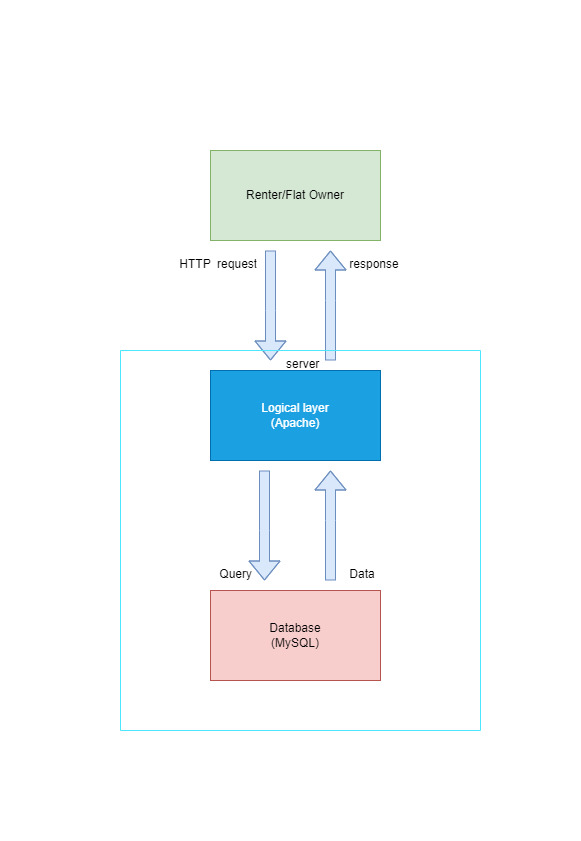
\includegraphics[width=1\textwidth,inner]{images/system.jpg}\\
\begin{center}
    Figure-4: System Architecture.
\end{center}
\end{center}
\clearpage

\section{Implementation}\label{sec:imp}
Here given some Data Definition Language(DDL) query which are used in our system\\
Listing~\ref{list:sql}   
\begin{lstlisting}[caption={ A SQL command for Creating table named USERS}, label=list:sql, captionpos=b,
           backgroundcolor=\color{white},
           language=SQL,
           breaklines=true,
           frame=single,
           showspaces=false,
           basicstyle=\ttfamily,
           numbers=left,
           numberstyle=\tiny,
           rulecolor=\color{red},
           keywordstyle=\color{blue},
           commentstyle=\color{gray}
        ]
CREATE TABLE users (
  ID int(16) UNSIGNED NOT NULL,
  username varchar(60) COLLATE utf8_unicode_ci NOT NULL,
  email varchar(255) COLLATE utf8_unicode_ci NOT NULL,
  password varchar(60) COLLATE utf8_unicode_ci NOT NULL,
  role varchar(60) COLLATE utf8_unicode_ci NOT NULL,
  name varchar(60) COLLATE utf8_unicode_ci NOT NULL,
  address varchar(250) COLLATE utf8_unicode_ci NOT NULL,
  phone varchar(14) COLLATE utf8_unicode_ci NOT NULL,
  date datetime NOT NULL
) ENGINE=InnoDB DEFAULT CHARSET=utf8 COLLATE=utf8_unicode_ci;
\end{lstlisting}

\begin{lstlisting}[caption={A SQL command for setting primary key. }, label=list:sql, captionpos=b,
           backgroundcolor=\color{white},
           language=SQL,
           breaklines=true,
           frame=single,
           showspaces=false,
           basicstyle=\ttfamily,
           numbers=left,
           numberstyle=\tiny,
           rulecolor=\color{red},
           keywordstyle=\color{blue},
           commentstyle=\color{gray}
        ]		 
 ALTER TABLE flat_info
  ADD PRIMARY KEY (ID);
\end{lstlisting}
\begin{lstlisting}[caption={A SQL command for setting primary key.}, label=list:sql, captionpos=b,
           backgroundcolor=\color{white},
           language=SQL,
           breaklines=true,
           frame=single,
           showspaces=false,
           basicstyle=\ttfamily,
           numbers=left,
           numberstyle=\tiny,
           rulecolor=\color{red},
           keywordstyle=\color{blue},
           commentstyle=\color{gray}
           ]
ALTER TABLE users
  ADD PRIMARY KEY (ID);
\end{lstlisting}
\begin{lstlisting}[caption={A SQL command for Creating table named booking-info}, label=list:sql, captionpos=b,
           backgroundcolor=\color{white},
           language=SQL,
           breaklines=true,
           frame=single,
           showspaces=false,
           basicstyle=\ttfamily,
           numbers=left,
           numberstyle=\tiny,
           rulecolor=\color{red},
           keywordstyle=\color{blue},
           commentstyle=\color{gray}
           ]
CREATE TABLE bookinginfo (
  bookID int(16) UNSIGNED NOT NULL,
  userID int(16) UNSIGNED NOT NULL,
  flatID int(16) UNSIGNED NOT NULL,
  date datetime NOT NULL
) ENGINE=InnoDB DEFAULT CHARSET=utf8 COLLATE=utf8_unicode_ci;
\end{lstlisting}
\begin{lstlisting}[caption={A SQL command for Creating table named Flat-info}, label=list:sql, captionpos=b,
           backgroundcolor=\color{white},
           language=SQL,
           breaklines=true,
           frame=single,
           showspaces=false,
           basicstyle=\ttfamily,
           numbers=left,
           numberstyle=\tiny,
           rulecolor=\color{red},
           keywordstyle=\color{blue},
           commentstyle=\color{gray}
           ]
CREATE TABLE flatinfo (
  flatID int(16) UNSIGNED NOT NULL,
  userID int(16) UNSIGNED NOT NULL,
  status enum('Available','Booked','Trash') COLLATE utf8_unicode_ci DEFAULT 'Available',
  type enum('Flat','Mess','Cottage') COLLATE utf8_unicode_ci DEFAULT 'Flat',
  floor varchar(10) COLLATE utf8_unicode_ci NOT NULL,
  rent int(10) NOT NULL,
  room varchar(20) COLLATE utf8_unicode_ci NOT NULL,
  address varchar(250) COLLATE utf8_unicode_ci NOT NULL,
  mobile varchar(15) COLLATE utf8_unicode_ci NOT NULL,
  facID int(16) UNSIGNED NOT NULL,
  date datetime NOT NULL,
  images longtext COLLATE utf8_unicode_ci NOT NULL
) ENGINE=InnoDB DEFAULT CHARSET=utf8 COLLATE=utf8_unicode_ci;
\end{lstlisting}
\begin{lstlisting}[caption={A SQL command for Creating table named logInfo}, label=list:sql, captionpos=b,
           backgroundcolor=\color{white},
           language=SQL,
           breaklines=true,
           frame=single,
           showspaces=false,
           basicstyle=\ttfamily,
           numbers=left,
           numberstyle=\tiny,
           rulecolor=\color{red},
           keywordstyle=\color{blue},
           commentstyle=\color{gray}
           ]
 CREATE TABLE loginfo (
  logID int(16) UNSIGNED NOT NULL,
  userID int(16) UNSIGNED NOT NULL,
  ipAddress varchar(15) COLLATE utf8_unicode_ci DEFAULT NULL,
  os varchar(10) COLLATE utf8_unicode_ci DEFAULT NULL,
  browser varchar(20) COLLATE utf8_unicode_ci DEFAULT NULL,
  date datetime NOT NULL
) ENGINE=InnoDB DEFAULT CHARSET=utf8 COLLATE=utf8_unicode_ci;
\end{lstlisting}


\begin{lstlisting}[caption={A SQL command for Creating table named user-role}, label=list:sql, captionpos=b,
           backgroundcolor=\color{white},
           language=SQL,
           breaklines=true,
           frame=single,
           showspaces=false,
           basicstyle=\ttfamily,
           numbers=left,
           numberstyle=\tiny,
           rulecolor=\color{red},
           keywordstyle=\color{blue},
           commentstyle=\color{gray}
           ]
SELECT * FROM user_role WHERE roleID = '$role_Id';
           
\end{lstlisting}

\begin{lstlisting}[caption={A SQL command for  connecting   logInfo and user }, label=list:sql, captionpos=b,
           backgroundcolor=\color{white},
           language=SQL,
           breaklines=true,
           frame=single,
           showspaces=false,
           basicstyle=\ttfamily,
           numbers=left,
           numberstyle=\tiny,
           rulecolor=\color{red},
           keywordstyle=\color{blue},
           commentstyle=\color{gray}
           ]
 SELECT user.*, loginfo.logID, loginfo.userID FROM loginfo    RIGHT JOIN user on loginfo.userID = user.userID WHERE       loginfo.logID = '$logID' AND loginfo.securityKey='$logKey;
           
\end{lstlisting}

\begin{lstlisting}[caption={A SQL command for  connecting     flatinfo  and facilities }, label=list:sql, captionpos=b,
           backgroundcolor=\color{white},
           language=SQL,
           breaklines=true,
           frame=single,
           showspaces=false,
           basicstyle=\ttfamily,
           numbers=left,
           numberstyle=\tiny,
           rulecolor=\color{red},
           keywordstyle=\color{blue},
           commentstyle=\color{gray}
           ]
 SELECT flatinfo.*, facilities.*, facilities.facID AS facID   FROM flatinfo LEFT JOIN facilities ON flatinfo.facID =      facilities.facID ORDER BY date ASC;
           
\end{lstlisting}

%ccccc
\begin{lstlisting}[caption={A SQL command for deleting     flatinfo  }, label=list:sql, captionpos=b,
           backgroundcolor=\color{white},
           language=SQL,
           breaklines=true,
           frame=single,
           showspaces=false,
           basicstyle=\ttfamily,
           numbers=left,
           numberstyle=\tiny,
           rulecolor=\color{red},
           keywordstyle=\color{blue},
           commentstyle=\color{gray}
           ]
 DELETE FROM flatinfo WHERE userID='$user_id' AND flatID='$id';
           
\end{lstlisting}

 
\begin{lstlisting}[caption={A SQL command for  Setting status     flatinfo  }, label=list:sql, captionpos=b,
           backgroundcolor=\color{white},
           language=SQL,
           breaklines=true,
           frame=single,
           showspaces=false,
           basicstyle=\ttfamily,
           numbers=left,
           numberstyle=\tiny,
           rulecolor=\color{red},
           keywordstyle=\color{blue},
           commentstyle=\color{gray}
           ]
 UPDATE flatinfo SET status='Booked', bookedUser='$user_i' WHERE flatID='$id' AND userID='$user_id';
           
\end{lstlisting}

\begin{lstlisting}[caption={A SQL command for updating status  flatinfo  }, label=list:sql, captionpos=b,
           backgroundcolor=\color{white},
           language=SQL,
           breaklines=true,
           frame=single,
           showspaces=false,
           basicstyle=\ttfamily,
           numbers=left,
           numberstyle=\tiny,
           rulecolor=\color{red},
           keywordstyle=\color{blue},
           commentstyle=\color{gray}
           ]
 UPDATE flatinfo SET status='Available', bookedUser=NULL      WHERE flatID='$id' AND userID='$user_id';
           
\end{lstlisting}

\begin{lstlisting}[caption={A SQL command for finding username from user table }, label=list:sql, captionpos=b,
           backgroundcolor=\color{white},
           language=SQL,
           breaklines=true,
           frame=single,
           showspaces=false,
           basicstyle=\ttfamily,
           numbers=left,
           numberstyle=\tiny,
           rulecolor=\color{red},
           keywordstyle=\color{blue},
           commentstyle=\color{gray}
           ]
SELECT * FROM user WHERE username='$username';
           
\end{lstlisting}

\begin{lstlisting}[caption={A SQL command for update user }, label=list:sql, captionpos=b,
           backgroundcolor=\color{white},
           language=SQL,
           breaklines=true,
           frame=single,
           showspaces=false,
           basicstyle=\ttfamily,
           numbers=left,
           numberstyle=\tiny,
           rulecolor=\color{red},
           keywordstyle=\color{blue},
           commentstyle=\color{gray}
           ]
 UPDATE user SET password='$password', email='$email',roleID='$type', name='$name', address='$address',phone='$phone' WHERE userID='$uid';
           
\end{lstlisting}

          
\\
\section{Validation} \label{sec:val}
\textbf{A simple user manual: }
When the user starts the application, he/she will find the landing page. A snap of lading page is given below. From this page, a user can go to login form or registration form.\\
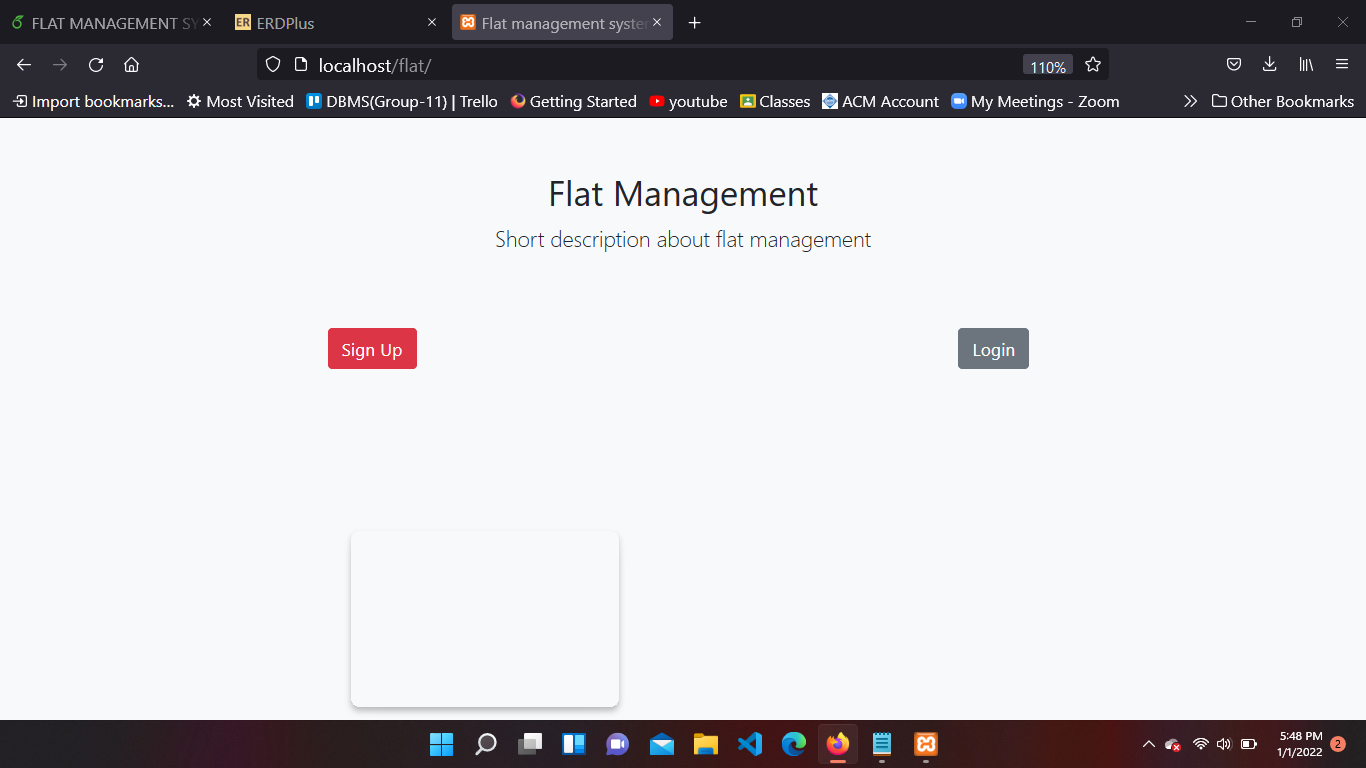
\includegraphics[width=1\textwidth, inner]{images/flat1.png}\\
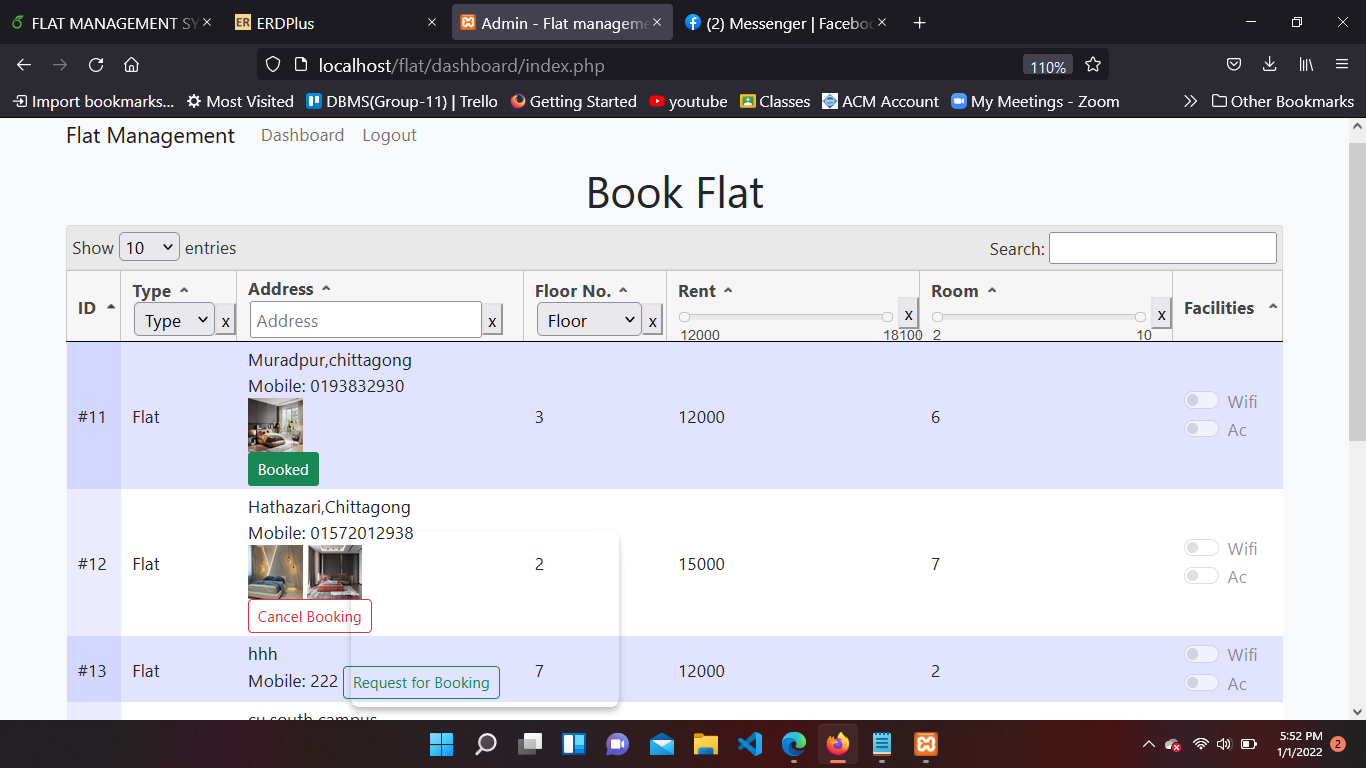
\includegraphics[width=1\textwidth, inner]{images/flat2.png}\\
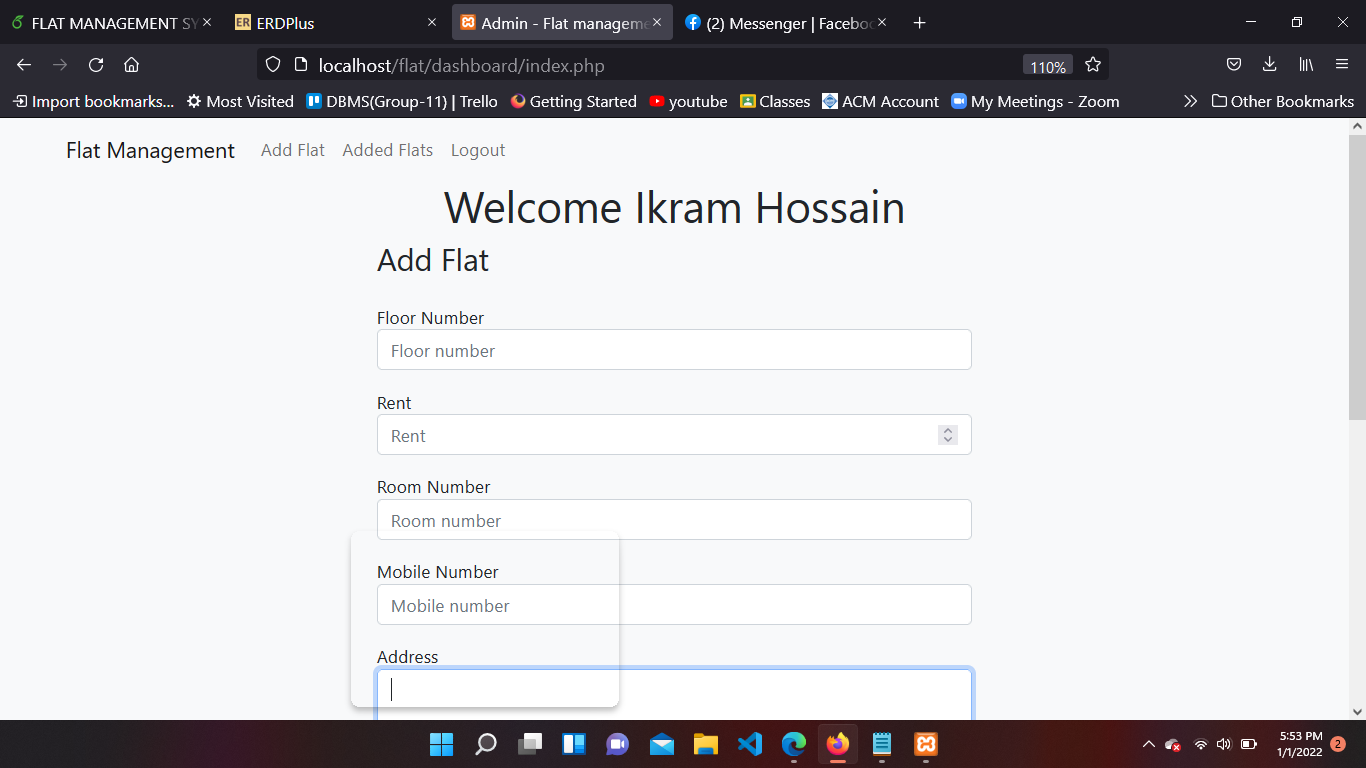
\includegraphics[width=1\textwidth, inner]{images/flat3.png}\\
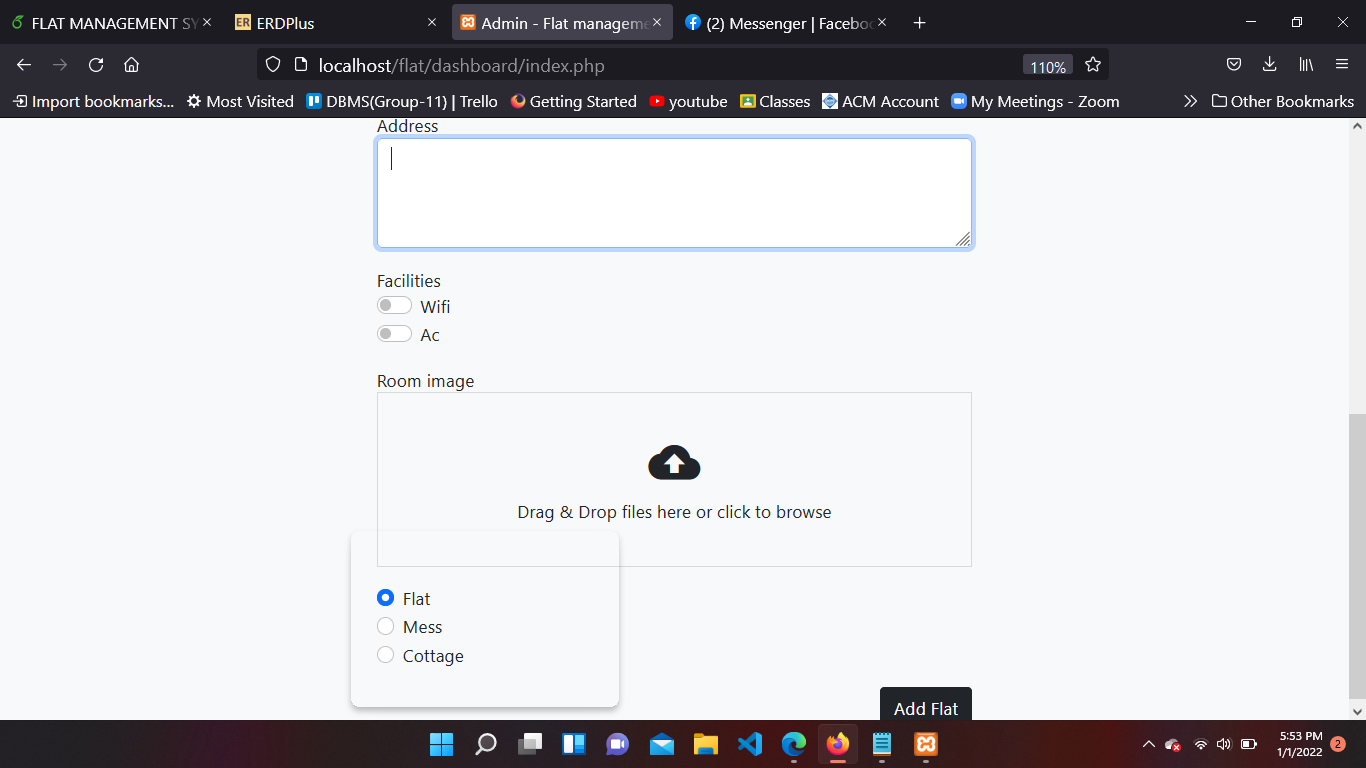
\includegraphics[width=1\textwidth, inner]{images/flat4.png}\\
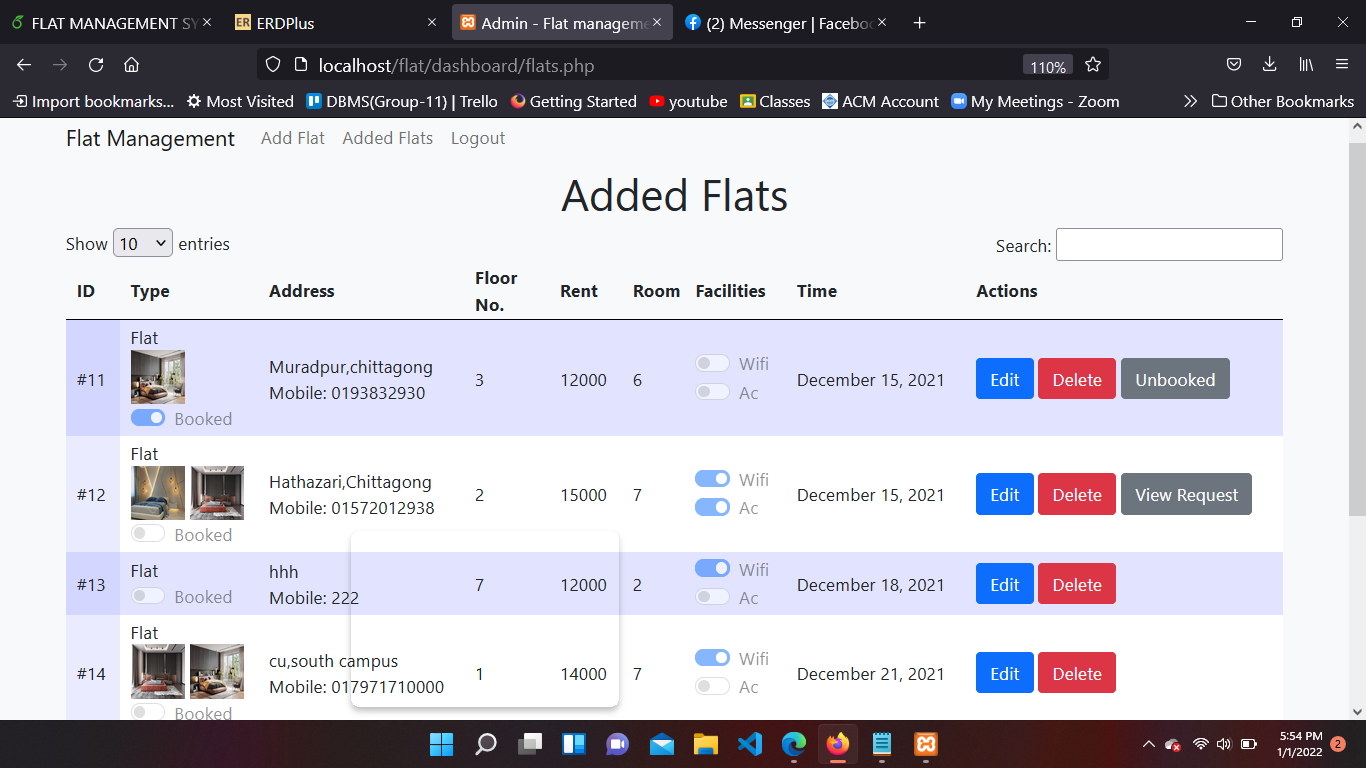
\includegraphics[width=1\textwidth, inner]{images/flat5.png}\\
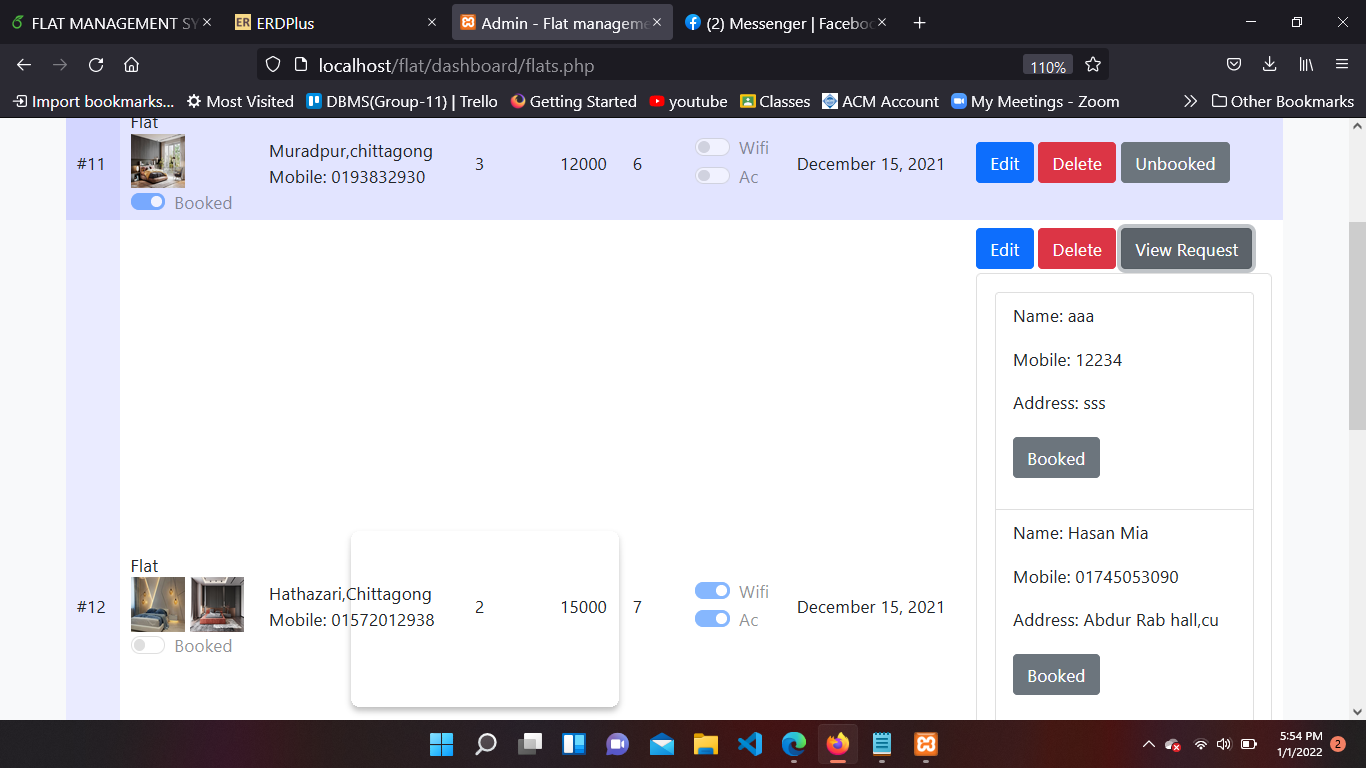
\includegraphics[width=1\textwidth, inner]{images/flat6.png}\\
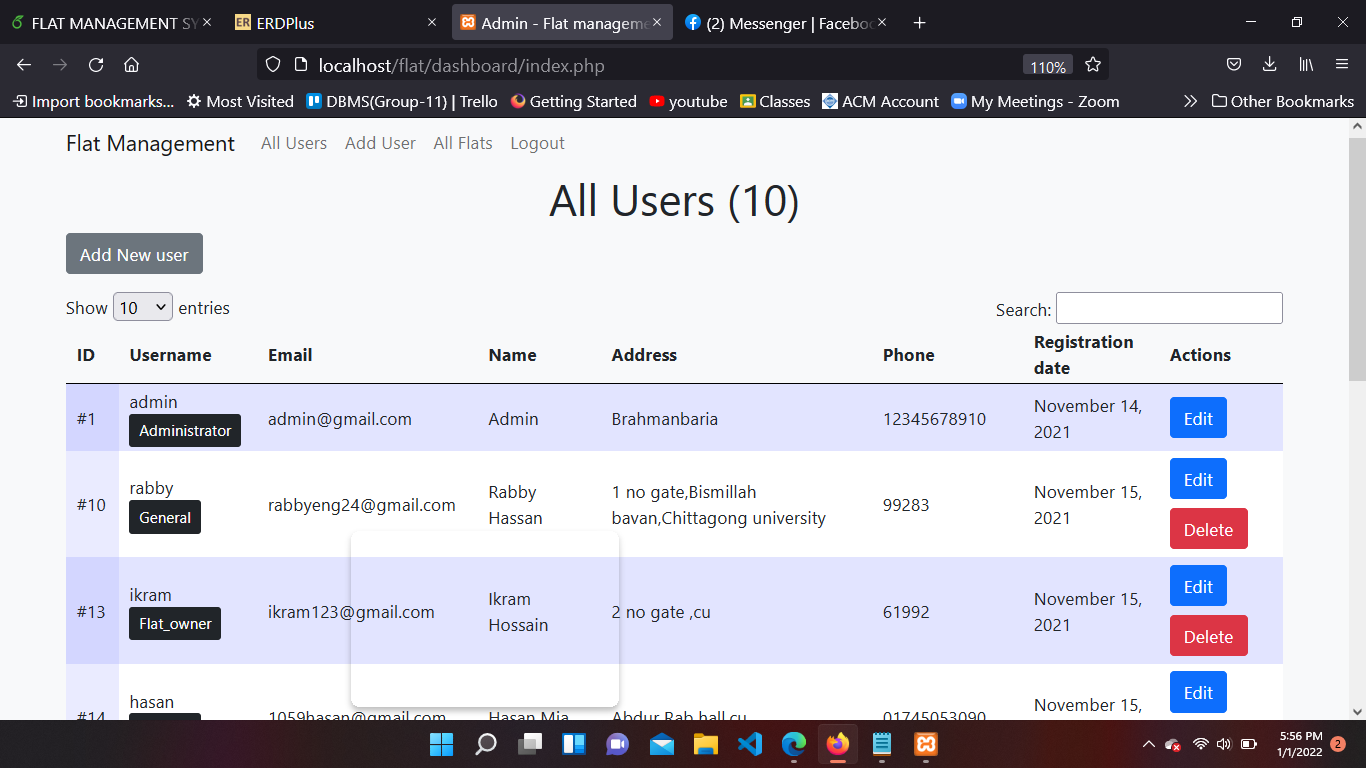
\includegraphics[width=1\textwidth, inner]{images/flat7.png}\\
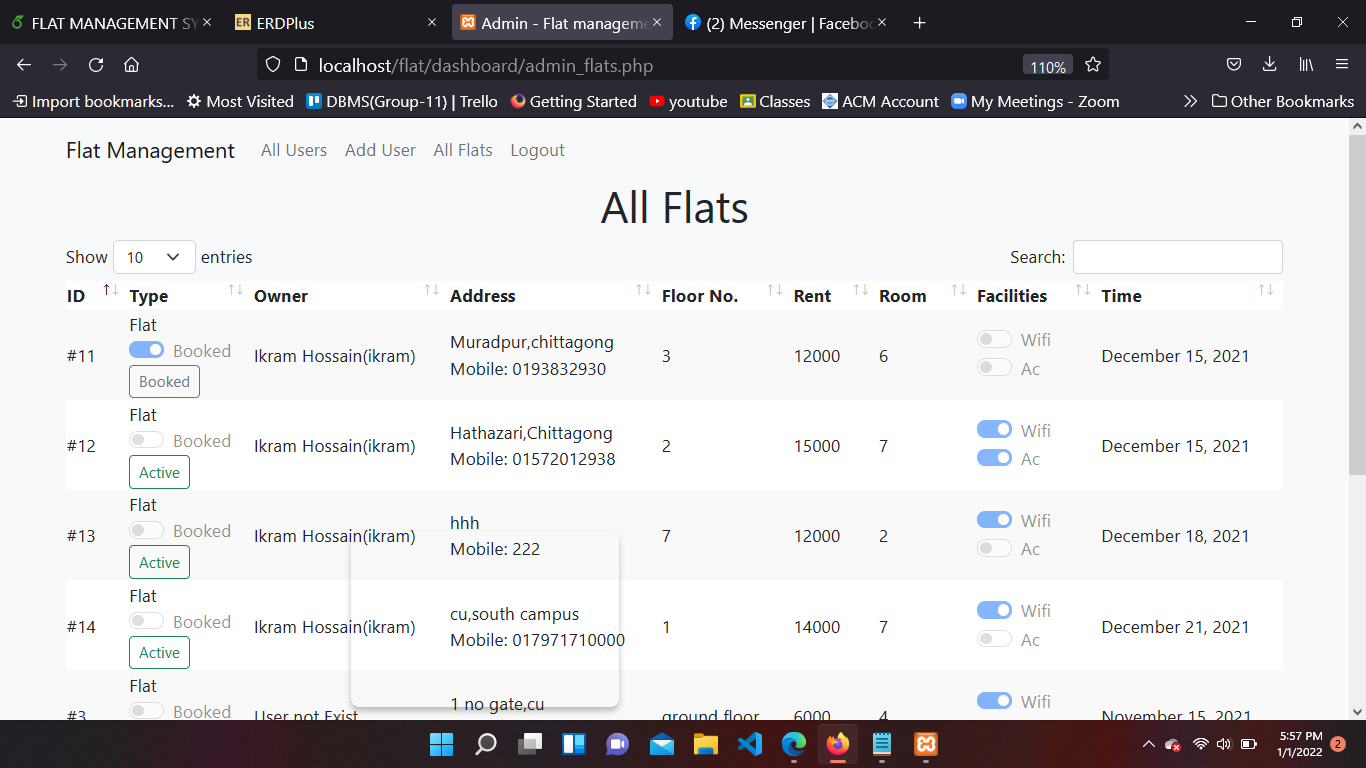
\includegraphics[width=1\textwidth, inner]{images/flat8.png}\\
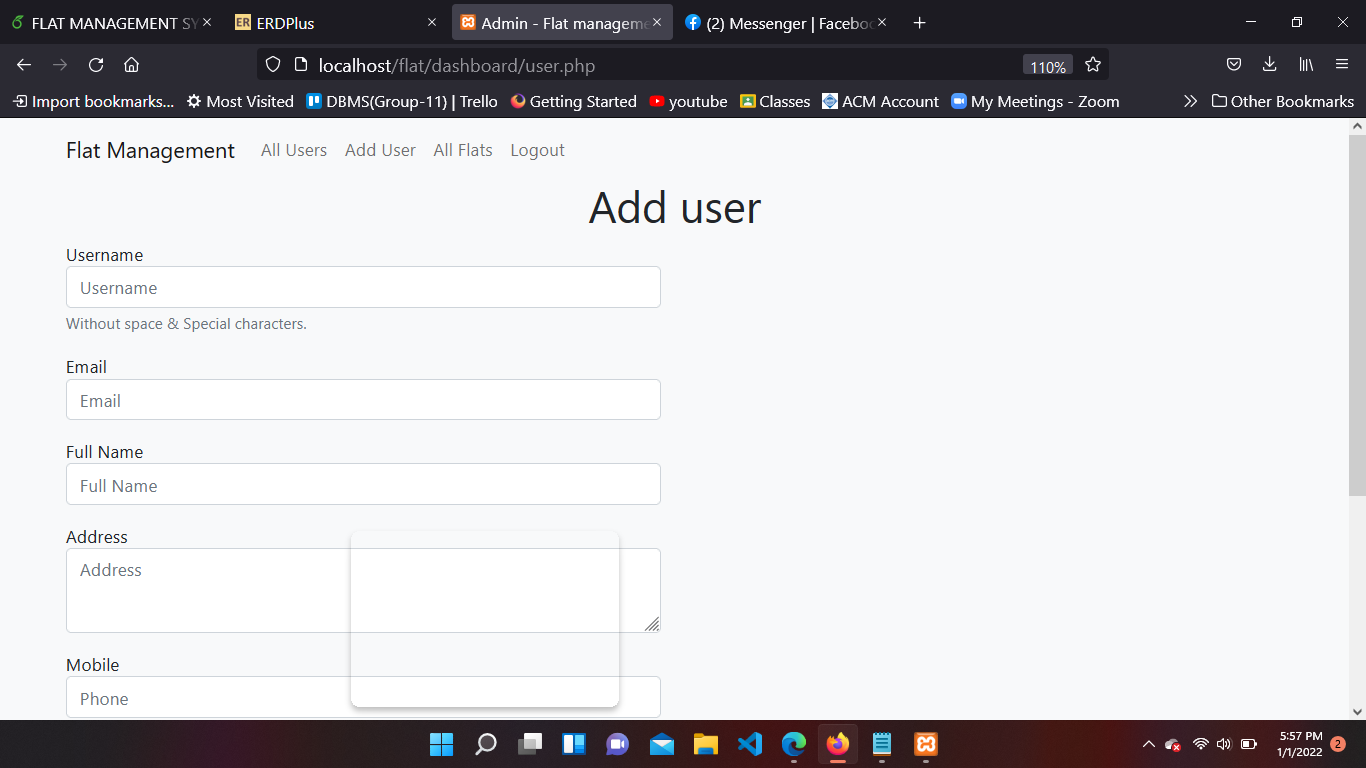
\includegraphics[width=1\textwidth, inner]{images/flat9.png}\\
 
\clearpage
\section{Software Deployment}\label{sec:sd}
\subsection{Server setting up}
 We have used localhost, Apache can be the best option for this. Firstly we have to
configure XAMPP with Apache and Mysql.
 \subsection{Database setting up}
After that we have to copy our database in phpMyadmin using exported sql
command.
 \subsection{Creating shortcut}

Then we can run our php files in browser.For general user we can create short-
cut for this system which will appear in home screen of the users device.

\subsection{ Run the application}
Finally any non-technical user can run this application by clicking the created
shortcut. 

\clearpage
\section{Conclusion and Future Work}\label{sec:cfw}
We wish that our Flat Management System will be user friendly. So we want to add a payment system to our Flat Management System in future. Besides this we want to activate messaging service in our project. Furthermore we want to add a review and a rating system so that users can express their opinion.
\clearpage




\section{Bibliography} 
\label{sec:bibliography}
~\cite{beighley2007head}
%\input{bibliography}
~\cite{silberschatz1997database}
~\cite{watson2008oca}






%\bibliographystyle{ios1}

\bibliographystyle{plain}
\bibliography{Bibliography.bib}




\end{document}